\begin{ledgroupsized}[r]{120mm}
\footnotesize
\pstart
\noindent\textbf{Überlieferung:}
\pend
\end{ledgroupsized}
\begin{ledgroupsized}[r]{114mm}
\footnotesize
\pstart \parindent -6mm
\makebox[6mm][l]{\textit{L}}%
Konzept:
LH~XXXV~11, 14~Bl.~36. 
Ein Blatt~8\textsuperscript{o};
oberer und linker Rand beschnitten.
Zwei Seiten; Textfolge: Bl.~36~v\textsuperscript{o}, Bl.~36~r\textsuperscript{o}.
Gemeinsame Schnittkanten mit LH~XXXV~4, 6~Bl.~12 und LH~XXXV~4, 6~Bl.~49.
\pend
\end{ledgroupsized}
\vspace{5mm}
\begin{ledgroup}
\footnotesize
\pstart
\noindent%
\textbf{Datierungsgründe:}
Zusammen mit LH~XXXV~4, 6~Bl.~12 und LH~XXXV~4, 6~Bl.~49 
(beide Stücke werden in Reihe VII erscheinen und sind bisher nicht datiert) bildete der Träger von N.\;\ref{58951} ein Quartblatt.
Auf LH~XXXV~4, 6~Bl.~49 befindet sich die Hälfte eines
nach aktuellem Kenntnisstand
für den Zeitraum Oktober 1690 bis März 1698 mehrfach belegten Wasserzeichens. %
\pend
\pstart
Im letzten Absatz von N.\;\ref{58951} kündigt Leibniz weitere Untersuchungen des schiefen Stoßes eines Körpers auf eine Mehrzahl anderer Körper an. Entsprechende Stellen finden sich in den Konzepten
N.\;\ref{41780} (bes. \refpassage{37_03_067_5a}{37_03_067_5b}),
und N.\;\ref{58300} (bes. \refpassage{35_13_03_242_6a}{35_13_03_242_6b})
die nach bisherigem Kenntnisstand auf die Zeiträume Januar 1691 bis 7.~Februar 1696 bzw.
Mitte September 1690 bis 1696 datierbar sind.
Demnach wird für die Entstehung von N.\;\ref{58951} das Ende der genannten Zeiträume als Terminus ante quem angenommen, woraus sich die angegebene Datierungsspanne ergibt.
\pend 
\end{ledgroup}
\selectlanguage{latin}
\vspace{8mm}
\pstart%
\normalsize%
\noindent%
\href{\Scan{LH_35_11_14_036v}}%
{\lbrack 36~v\textsuperscript{o}\rbrack}
\pend
\nobreak\begin{edfigure}[0.25em]%
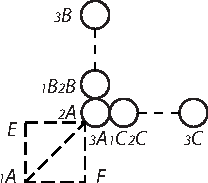
\includegraphics[scale=1]{gesamttex/edit_VIII-4/images/LH_35_11_14_036_d1_036v.pdf}
\edcaption{\edtext{\lbrack\textit{Fig.~1}\rbrack}{%
\lemma{\lbrack\textit{Fig.~1}\rbrack}%
\Cfootnote[nonum]{%
Ein gestrichener Entwurf zum Diagramm wird nicht wiedergegeben.}}}
\end{edfigure}
\pstart
\noindent
Si globus\indexS{globus}\indexS{globus in globos quiescentes incurrens} 
\textit{A} incurrat in globos\indexS{globus} \textit{B}, \textit{C}, 
\edtext{quiescentes videndum}{\lemma{quiescentes}\Bfootnote{%
\textit{(1)}~verum non est %
\textit{(2)}~videndum ~\textit{L}}} 
\textit{B} ire in \textit{\ind{3}B}, celeritate \textit{\ind{2}B\ind{3}B} $=$ \textit{F\ind{2}A} 
et \textit{C} ire in \textit{\ind{3}C} celeritate \textit{\ind{2}C\ind{3}C} $=$ \textit{E\ind{2}A}.
Sane hoc 
\edtext{modo manet}{\lemma{modo}\Bfootnote{%
\textit{(1)}~retinetur ea %
\textit{(2)}~manet~\textit{L}}} 
eadem vis directrix\indexS{vis directrix} 
\edtext{seu via centri,\indexS{via centri}}{\lemma{}\Bfootnote{seu via centri \textit{erg.~L}}}
et manet quoque eadem vis absoluta\indexS{vis absoluta}; ob summam 
\edtext{quadratorum.\indexS{summa quadratorum} Sed}{\lemma{quadratorum.}\Bfootnote{%
\textit{(1)}~Sed tamen arbitror hoc non procedere, quia non manet eadem quae ante vis respectiva, 
\bars{sed augetur \textit{streicht Hrsg.}} 
\textit{(2)}~Sed~\textit{L}}} 
quia haec data rem non determinant, ideo aliud quiddam adjiciendum, ut scil.\ eadem quoque %
vis respectiva\indexS{vis respectiva} colligi possit. Verum hac ratione video augeri vim respectivam,%
\indexS{vis respectiva} nam manet
\edtext{sic}{%
\lemma{}%
\Bfootnote{%
sic %
\textit{erg.~L}}}
eadem quae prior inter \textit{A} et \textit{BC}
cum eadem hoc modo sit 
\edtext{distantiarum augmentatio seu}{\lemma{distantiarum}\Bfootnote{%
\textit{(1)}~jam %
\textit{(2)}~augmentatio %
\textit{(a)}~inter %
\textit{(b)}~seu~\textit{L}}} 
celeritas respectiva\indexS{celeritas respectiva} inter
\edtext{\textit{A} et \lbrack\textit{D}\rbrack\ centrum}{%
\lemma{\textit{A} et}%
\Bfootnote{%
\textit{(1)}~\textit{D}
\textit{(2)}~\bars{\textit{C} \textit{ändert Hrsg.}} %
centrum
\textit{L}}}
gravitatis\indexS{centrum gravitatis} ipsorum \textit{BC}. Verum alia praeterea 
\edtext{adest vis\indexS{vis respectiva} respectiva}{\lemma{adest}\Bfootnote{%
\textit{(1)}~celeritas respectiva %
\textit{(2)}~vis respectiva~\textit{L}}} 
nova inter \textit{B} et 
\edtext{\textit{C}, invicem}{%
\lemma{\textit{C},}%
\Bfootnote{%
\textit{(1)}~quae pro %
\textit{(2)}~invicem~\textit{L}}}
discedentibus, ita lucrati fuissemus vim respectivam,%
\indexS{vis respectiva} quod absurdum est. Itaque non satis fidendum motuum compositioni\indexS{compositio motuum} 
nisi considerationi virium\indexS{vis}\indexS{consideratio virium} 
coincidat. 
\pend
\begin{edfigure}%
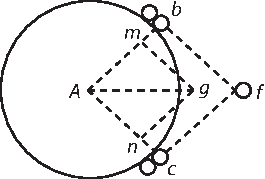
\includegraphics[scale=1]{gesamttex/edit_VIII-4/images/LH_35_11_14_036_d2_036v.pdf} 
\edcaption{%
\edtext{\lbrack\textit{Fig.~2}\rbrack}{%
\lemma{\lbrack\textit{Fig.~2}\rbrack}%
\Cfootnote[nonum]{Ein gestrichener Entwurf zum Diagramm wird nicht wiedergegeben.}}}
\end{edfigure}
\pstart
Sic si \textit{A} incidat simul in \textit{b} et \textit{c} sitque celeritas\indexS{celeritas composita}
\edtext{$A\lbrack f\rbrack$,}{%
\lemma{}%
\Bfootnote{%
\textit{AF}, %
\textit{L ändert Hrsg.}%
}}
 composita ex \textit{Ab} et \textit{Ac}, si igitur 
\edtext{perinde rem esse}{\lemma{perinde}\Bfootnote{%
\textit{(1)}~affici \textit{A} 
\textit{(2)}~rem esse~\textit{L}}} 
ponamus ac si simul \textit{A} incurrisset in \textit{b} celeritate \textit{Ab} et in \textit{c} celeritate \textit{Ac}, res eodem redibit 
\edtext{quoad \textit{A},}{\lemma{}\Bfootnote{quoad \textit{A} \textit{erg.~L}}}
ac si \textit{A} eadem quam dabat celeritate in unum eorum incurrisset, nam ex celeritatibus \textit{Ab}, \textit{Ac} fiet \textit{Am}, \textit{An}, cum ex \textit{Af}, fiat \textit{Ag} eadem proportione scil. $Am:Ab\squaredots Ag:Af\squaredots A-f,:A+f$. \pend
\pstart\noindent
\href{\Scan{LH_35_11_14_036r}}%
{\lbrack 36~r\textsuperscript{o}\rbrack} 
\pend
\nobreak
\begin{edfigure}[0.5em]%
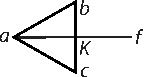
\includegraphics[scale=1]{gesamttex/edit_VIII-4/images/LH_35_11_14_036_d3_036r.pdf} 
\edcaption{\lbrack\textit{Fig.~3}\rbrack}
\end{edfigure}
\pstart
Considerandum etiam, si ponamus celeritatem \textit{af} compositam\indexS{celeritas composita} ex celeritatibus \textit{ab}, \textit{ac}, posito \textit{abfc} esse parallelogrammum;%
\indexS{parallelogrammum} in absoluta virium aestimatione%
\indexS{vis}\indexS{aestimatio absoluta virium} 
rem non procedere, 
\edtext{etiam}{\lemma{}\Bfootnote{etiam \textit{erg.~L}}}
 si ponamus esse rhombum%
\indexS{rhombus} seu $ab=ac=bf=cf$. Nam si 
\edtext{ponamus motum \textit{ab}}{\lemma{ponamus}\Bfootnote{%
\textit{(1)}~\textit{ab} 
\textit{(2)}~motum \textit{ab}~\textit{L}}} 
\edtext{componi ex $aK+Kb$,}{\lemma{}\Bfootnote{componi ex \textit{aK} \bars{et \textit{streicht Hrsg.}} $+\,Kb$,~\textit{L}}}
et 
\edtext{motum \textit{ac} ex}{\lemma{motum \textit{ac}}\Bfootnote{%
\textit{(1)}~ex \textit{aK} et \textit{Kb}, fiet quidem $aK-a$ %
\textit{(2)}~ex~\textit{L}}} 
$aK+Kc$
\edtext{seu ex $aK-\lbrack Kb\rbrack$ seu}{\lemma{}\Bfootnote{seu ex $aK\,-$ \bars{\textit{bK}  \textit{ändert Hrsg.}} seu~\textit{L}}}
ex 
\edtext{$Kf-\lbrack Kb\rbrack$, habemus}{\lemma{}\Bfootnote{$Kf\,-$ \bars{\textit{bK} \textit{ändert Hrsg.}} , habemus~\textit{L}}}
quidem $aK+Kb-Kb+Kf$, sed tamen praeterquam quod haec compositio%
\indexS{compositio motuum} non procedit in non rhombis,%
\indexS{rhombus} non tamen succedit virium compositio\indexS{compositio virium}, nam vires\indexS{vis} sunt $aK^2+Kb^2+aK^2$
\edtext{$+Kc^2$, seu bis}{\lemma{$+Kc^2$}\Bfootnote{%
\textit{(1)}~quae tamen non dant \textit{aK} %
\textit{(2)}~se %
\textit{(a)}~$2\cdot aK^2+$ %
\textit{(b)}~bis $aK^2$ %
\textit{(c)}~bis~\textit{L}}}
 $aK^2+\text{bis }bK^2$. Sed hoc non consentit cum quadrato ab \textit{af} quod est $4aK^2$ nisi eo solo casu cum %
rhombus\indexS{rhombus} abit in quadratum.%
\indexS{quadratum} 
\pend
\pstart
\edtext{Videndum quod fiat, cum globus unus 
\edtext{incurrit amphidextre}{%
\lemma{incurrit}%
\Bfootnote{%
\textit{(1)}~ambidextre %
\textit{(2)}~amphidextre~\textit{L}}}
in plures,%
\indexS{globus unus amphidextre in plures incurrens} item cum globus incurrit in globum plures amphidextre tangentem.\indexS{globus plures globos amphidextre tangens}
Possunt plures rursus tangi a paucioribus et semper paucioribus donec res reducitur ad unum. Ita plura notabilia colligentur.%
}{\lemma{Videndum \lbrack...\rbrack\  colligentur}%
\Cfootnote{%
Entsprechende Untersuchungen werden in den Konzepten N.\;\ref{41780} (bes. \refpassage{37_03_067_5a}{37_03_067_5b}) und N.\;\ref{58300} (bes. \refpassage{35_13_03_242_6a}{35_13_03_242_6b}) angestellt.}}
\pend
